% Created by tikzDevice version 0.10.1 on 2018-03-04 17:10:26
% !TEX encoding = UTF-8 Unicode
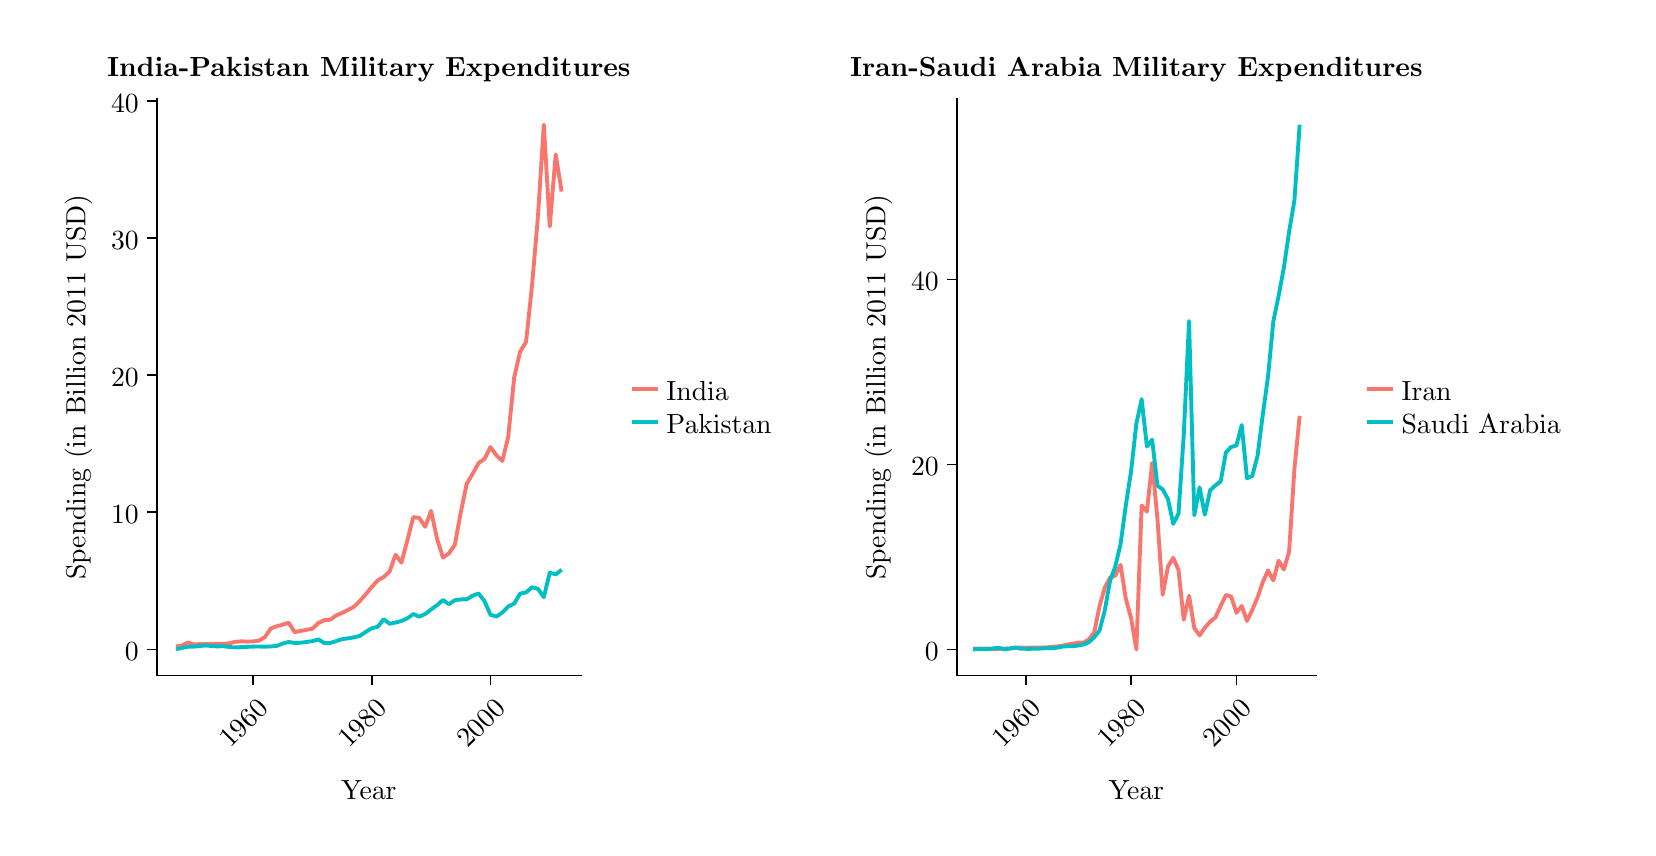
\begin{tikzpicture}[x=1pt,y=1pt]
\definecolor{fillColor}{RGB}{255,255,255}
\path[use as bounding box,fill=fillColor,fill opacity=0.00] (0,0) rectangle (578.16,289.08);
\begin{scope}
\path[clip] ( 46.64, 54.95) rectangle (199.91,263.47);
\definecolor{drawColor}{RGB}{248,118,109}

\path[draw=drawColor,line width= 1.4pt,line join=round] ( 53.60, 65.51) --
	( 55.75, 65.79) --
	( 57.89, 66.92) --
	( 60.03, 66.24) --
	( 62.18, 66.33) --
	( 64.32, 66.36) --
	( 66.47, 66.43) --
	( 68.61, 66.47) --
	( 70.75, 66.42) --
	( 72.90, 66.62) --
	( 75.04, 67.18) --
	( 77.18, 67.33) --
	( 79.33, 67.23) --
	( 81.47, 67.30) --
	( 83.62, 67.59) --
	( 85.76, 68.94) --
	( 87.90, 72.01) --
	( 90.05, 72.80) --
	( 92.19, 73.36) --
	( 94.33, 74.05) --
	( 96.48, 70.66) --
	( 98.62, 71.10) --
	(100.76, 71.48) --
	(102.91, 71.90) --
	(105.05, 73.96) --
	(107.20, 75.00) --
	(109.34, 75.14) --
	(111.48, 76.68) --
	(113.63, 77.60) --
	(115.77, 78.69) --
	(117.91, 79.83) --
	(120.06, 81.94) --
	(122.20, 84.36) --
	(124.35, 87.02) --
	(126.49, 89.30) --
	(128.63, 90.57) --
	(130.78, 92.57) --
	(132.92, 98.64) --
	(135.06, 95.78) --
	(137.21,103.90) --
	(139.35,112.22) --
	(141.49,111.92) --
	(143.64,108.70) --
	(145.78,114.45) --
	(147.93,104.39) --
	(150.07, 97.61) --
	(152.21, 99.10) --
	(154.36,102.26) --
	(156.50,113.91) --
	(158.64,124.25) --
	(160.79,127.84) --
	(162.93,131.75) --
	(165.08,133.24) --
	(167.22,137.55) --
	(169.36,134.59) --
	(171.51,132.52) --
	(173.65,141.23) --
	(175.79,162.59) --
	(177.94,172.02) --
	(180.08,175.50) --
	(182.23,195.73) --
	(184.37,220.63) --
	(186.51,254.00) --
	(188.66,217.28) --
	(190.80,243.28) --
	(192.94,229.86);
\definecolor{drawColor}{RGB}{0,191,196}

\path[draw=drawColor,line width= 1.4pt,line join=round] ( 53.60, 64.43) --
	( 55.75, 64.96) --
	( 57.89, 65.36) --
	( 60.03, 65.42) --
	( 62.18, 65.64) --
	( 64.32, 65.83) --
	( 66.47, 65.65) --
	( 68.61, 65.48) --
	( 70.75, 65.60) --
	( 72.90, 65.25) --
	( 75.04, 65.17) --
	( 77.18, 65.23) --
	( 79.33, 65.34) --
	( 81.47, 65.44) --
	( 83.62, 65.45) --
	( 85.76, 65.40) --
	( 87.90, 65.49) --
	( 90.05, 65.68) --
	( 92.19, 66.55) --
	( 94.33, 67.10) --
	( 96.48, 66.74) --
	( 98.62, 66.82) --
	(100.76, 67.10) --
	(102.91, 67.41) --
	(105.05, 68.03) --
	(107.20, 66.69) --
	(109.34, 66.76) --
	(111.48, 67.40) --
	(113.63, 68.14) --
	(115.77, 68.41) --
	(117.91, 68.78) --
	(120.06, 69.32) --
	(122.20, 70.76) --
	(124.35, 72.07) --
	(126.49, 72.59) --
	(128.63, 75.33) --
	(130.78, 73.70) --
	(132.92, 74.12) --
	(135.06, 74.67) --
	(137.21, 75.67) --
	(139.35, 77.21) --
	(141.49, 76.22) --
	(143.64, 77.21) --
	(145.78, 78.84) --
	(147.93, 80.42) --
	(150.07, 82.26) --
	(152.21, 80.77) --
	(154.36, 82.18) --
	(156.50, 82.47) --
	(158.64, 82.51) --
	(160.79, 83.82) --
	(162.93, 84.62) --
	(165.08, 81.88) --
	(167.22, 76.92) --
	(169.36, 76.29) --
	(171.51, 77.74) --
	(173.65, 79.92) --
	(175.79, 80.96) --
	(177.94, 84.57) --
	(180.08, 85.01) --
	(182.23, 86.86) --
	(184.37, 86.33) --
	(186.51, 83.30) --
	(188.66, 92.16) --
	(190.80, 91.51) --
	(192.94, 93.22);
\end{scope}
\begin{scope}
\path[clip] (  0.00,  0.00) rectangle (578.16,289.08);
\definecolor{drawColor}{RGB}{0,0,0}

\path[draw=drawColor,line width= 0.6pt,line join=round,line cap=rect] ( 46.64, 54.95) --
	( 46.64,263.47);
\end{scope}
\begin{scope}
\path[clip] (  0.00,  0.00) rectangle (578.16,289.08);
\definecolor{drawColor}{RGB}{0,0,0}

\node[text=drawColor,anchor=base east,inner sep=0pt, outer sep=0pt, scale=  1.0000] at ( 40.14, 60.30) {0};

\node[text=drawColor,anchor=base east,inner sep=0pt, outer sep=0pt, scale=  1.0000] at ( 40.14,109.82) {10};

\node[text=drawColor,anchor=base east,inner sep=0pt, outer sep=0pt, scale=  1.0000] at ( 40.14,159.34) {20};

\node[text=drawColor,anchor=base east,inner sep=0pt, outer sep=0pt, scale=  1.0000] at ( 40.14,208.87) {30};

\node[text=drawColor,anchor=base east,inner sep=0pt, outer sep=0pt, scale=  1.0000] at ( 40.14,258.39) {40};
\end{scope}
\begin{scope}
\path[clip] (  0.00,  0.00) rectangle (578.16,289.08);
\definecolor{drawColor}{RGB}{0,0,0}

\path[draw=drawColor,line width= 0.6pt,line join=round] ( 43.14, 64.43) --
	( 46.64, 64.43);

\path[draw=drawColor,line width= 0.6pt,line join=round] ( 43.14,113.95) --
	( 46.64,113.95);

\path[draw=drawColor,line width= 0.6pt,line join=round] ( 43.14,163.48) --
	( 46.64,163.48);

\path[draw=drawColor,line width= 0.6pt,line join=round] ( 43.14,213.00) --
	( 46.64,213.00);

\path[draw=drawColor,line width= 0.6pt,line join=round] ( 43.14,262.52) --
	( 46.64,262.52);
\end{scope}
\begin{scope}
\path[clip] (  0.00,  0.00) rectangle (578.16,289.08);
\definecolor{drawColor}{RGB}{0,0,0}

\path[draw=drawColor,line width= 0.6pt,line join=round,line cap=rect] ( 46.64, 54.95) --
	(199.91, 54.95);
\end{scope}
\begin{scope}
\path[clip] (  0.00,  0.00) rectangle (578.16,289.08);
\definecolor{drawColor}{RGB}{0,0,0}

\path[draw=drawColor,line width= 0.6pt,line join=round] ( 81.47, 51.45) --
	( 81.47, 54.95);

\path[draw=drawColor,line width= 0.6pt,line join=round] (124.35, 51.45) --
	(124.35, 54.95);

\path[draw=drawColor,line width= 0.6pt,line join=round] (167.22, 51.45) --
	(167.22, 54.95);
\end{scope}
\begin{scope}
\path[clip] (  0.00,  0.00) rectangle (578.16,289.08);
\definecolor{drawColor}{RGB}{0,0,0}

\node[text=drawColor,rotate= 45.00,anchor=base east,inner sep=0pt, outer sep=0pt, scale=  1.0000] at ( 87.32, 42.61) {1960};

\node[text=drawColor,rotate= 45.00,anchor=base east,inner sep=0pt, outer sep=0pt, scale=  1.0000] at (130.19, 42.61) {1980};

\node[text=drawColor,rotate= 45.00,anchor=base east,inner sep=0pt, outer sep=0pt, scale=  1.0000] at (173.06, 42.61) {2000};
\end{scope}
\begin{scope}
\path[clip] (  0.00,  0.00) rectangle (578.16,289.08);
\definecolor{drawColor}{RGB}{0,0,0}

\node[text=drawColor,anchor=base,inner sep=0pt, outer sep=0pt, scale=  1.0000000] at (123.27, 10.00) {Year};
\end{scope}
\begin{scope}
\path[clip] (  0.00,  0.00) rectangle (578.16,289.08);
\definecolor{drawColor}{RGB}{0,0,0}

\node[text=drawColor,rotate= 90.00,anchor=base,inner sep=0pt, outer sep=0pt, scale=  1.0000000] at ( 20.89,159.21) {Spending (in Billion 2011 USD)};
\end{scope}
\begin{scope}
\path[clip] (  0.00,  0.00) rectangle (578.16,289.08);
\definecolor{drawColor}{RGB}{248,118,109}

\path[draw=drawColor,line width= 1.4pt,line join=round] (218.19,158.61) -- (227.82,158.61);
\end{scope}
\begin{scope}
\path[clip] (  0.00,  0.00) rectangle (578.16,289.08);
\definecolor{drawColor}{RGB}{0,191,196}

\path[draw=drawColor,line width= 1.4pt,line join=round] (218.19,146.56) -- (227.82,146.56);
\end{scope}
\begin{scope}
\path[clip] (  0.00,  0.00) rectangle (578.16,289.08);
\definecolor{drawColor}{RGB}{0,0,0}

\node[text=drawColor,anchor=base west,inner sep=0pt, outer sep=0pt, scale=  1.0000] at (230.83,154.47) {India};
\end{scope}
\begin{scope}
\path[clip] (  0.00,  0.00) rectangle (578.16,289.08);
\definecolor{drawColor}{RGB}{0,0,0}

\node[text=drawColor,anchor=base west,inner sep=0pt, outer sep=0pt, scale=  1.0000] at (230.83,142.43) {Pakistan};
\end{scope}
\begin{scope}
\path[clip] (  0.00,  0.00) rectangle (578.16,289.08);
\definecolor{drawColor}{RGB}{0,0,0}

\node[text=drawColor,anchor=base,inner sep=0pt, outer sep=0pt, scale=  1.0000000] at (123.27,271.45) {\bfseries India-Pakistan Military Expenditures};
\end{scope}
\begin{scope}
\path[clip] (335.72, 54.95) rectangle (465.53,263.47);
\definecolor{drawColor}{RGB}{248,118,109}

\path[draw=drawColor,line width= 1.4pt,line join=round] (341.62, 64.68) --
	(343.52, 64.68) --
	(345.42, 64.69) --
	(347.33, 64.69) --
	(349.23, 64.56) --
	(351.13, 64.62) --
	(353.04, 64.70) --
	(354.94, 64.77) --
	(356.84, 64.98) --
	(358.75, 65.11) --
	(360.65, 65.03) --
	(362.55, 65.05) --
	(364.46, 65.05) --
	(366.36, 65.07) --
	(368.26, 65.16) --
	(370.17, 65.35) --
	(372.07, 65.48) --
	(373.98, 65.80) --
	(375.88, 66.18) --
	(377.78, 66.52) --
	(379.69, 66.89) --
	(381.59, 66.89) --
	(383.49, 68.06) --
	(385.40, 70.49) --
	(387.30, 80.00) --
	(389.20, 86.71) --
	(391.11, 90.32) --
	(393.01, 91.07) --
	(394.91, 94.97) --
	(396.82, 82.69) --
	(398.72, 75.75) --
	(400.62, 64.43) --
	(402.53,116.40) --
	(404.43,114.23) --
	(406.33,131.81) --
	(408.24,111.52) --
	(410.14, 84.15) --
	(412.04, 94.37) --
	(413.95, 97.51) --
	(415.85, 93.17) --
	(417.75, 75.12) --
	(419.66, 83.81) --
	(421.56, 72.12) --
	(423.46, 69.50) --
	(425.37, 72.25) --
	(427.27, 74.45) --
	(429.17, 75.93) --
	(431.08, 80.12) --
	(432.98, 84.08) --
	(434.88, 83.51) --
	(436.79, 77.65) --
	(438.69, 80.13) --
	(440.59, 74.71) --
	(442.50, 78.70) --
	(444.40, 83.16) --
	(446.31, 88.74) --
	(448.21, 92.97) --
	(450.11, 89.33) --
	(452.02, 96.49) --
	(453.92, 93.29) --
	(455.82, 99.73) --
	(457.73,129.63) --
	(459.63,148.81);
\definecolor{drawColor}{RGB}{0,191,196}

\path[draw=drawColor,line width= 1.4pt,line join=round] (341.62, 64.43) --
	(343.52, 64.51) --
	(345.42, 64.49) --
	(347.33, 64.55) --
	(349.23, 64.84) --
	(351.13, 64.94) --
	(353.04, 64.43) --
	(354.94, 64.73) --
	(356.84, 65.11) --
	(358.75, 64.67) --
	(360.65, 64.63) --
	(362.55, 64.63) --
	(364.46, 64.67) --
	(366.36, 64.74) --
	(368.26, 64.84) --
	(370.17, 64.87) --
	(372.07, 65.03) --
	(373.98, 65.44) --
	(375.88, 65.55) --
	(377.78, 65.56) --
	(379.69, 65.85) --
	(381.59, 66.20) --
	(383.49, 67.05) --
	(385.40, 68.79) --
	(387.30, 71.21) --
	(389.20, 78.47) --
	(391.11, 89.20) --
	(393.01, 94.38) --
	(394.91,102.46) --
	(396.82,116.52) --
	(398.72,128.80) --
	(400.62,145.97) --
	(402.53,154.87) --
	(404.43,137.69) --
	(406.33,140.20) --
	(408.24,123.56) --
	(410.14,122.24) --
	(412.04,118.70) --
	(413.95,109.78) --
	(415.85,113.52) --
	(417.75,141.96) --
	(419.66,183.07) --
	(421.56,112.85) --
	(423.46,122.97) --
	(425.37,113.07) --
	(427.27,121.90) --
	(429.17,123.68) --
	(431.08,125.09) --
	(432.98,135.62) --
	(434.88,137.54) --
	(436.79,138.12) --
	(438.69,145.52) --
	(440.59,126.26) --
	(442.50,127.08) --
	(444.40,134.31) --
	(446.31,149.22) --
	(448.21,163.15) --
	(450.11,182.89) --
	(452.02,192.17) --
	(453.92,202.37) --
	(455.82,215.38) --
	(457.73,226.62) --
	(459.63,254.00);
\end{scope}
\begin{scope}
\path[clip] (  0.00,  0.00) rectangle (578.16,289.08);
\definecolor{drawColor}{RGB}{0,0,0}

\path[draw=drawColor,line width= 0.6pt,line join=round,line cap=rect] (335.72, 54.95) --
	(335.72,263.47);
\end{scope}
\begin{scope}
\path[clip] (  0.00,  0.00) rectangle (578.16,289.08);
\definecolor{drawColor}{RGB}{0,0,0}

\node[text=drawColor,anchor=base east,inner sep=0pt, outer sep=0pt, scale=  1.0000] at (329.22, 60.30) {0};

\node[text=drawColor,anchor=base east,inner sep=0pt, outer sep=0pt, scale=  1.0000] at (329.22,127.13) {20};

\node[text=drawColor,anchor=base east,inner sep=0pt, outer sep=0pt, scale=  1.0000] at (329.22,193.97) {40};
\end{scope}
\begin{scope}
\path[clip] (  0.00,  0.00) rectangle (578.16,289.08);
\definecolor{drawColor}{RGB}{0,0,0}

\path[draw=drawColor,line width= 0.6pt,line join=round] (332.22, 64.43) --
	(335.72, 64.43);

\path[draw=drawColor,line width= 0.6pt,line join=round] (332.22,131.27) --
	(335.72,131.27);

\path[draw=drawColor,line width= 0.6pt,line join=round] (332.22,198.11) --
	(335.72,198.11);
\end{scope}
\begin{scope}
\path[clip] (  0.00,  0.00) rectangle (578.16,289.08);
\definecolor{drawColor}{RGB}{0,0,0}

\path[draw=drawColor,line width= 0.6pt,line join=round,line cap=rect] (335.72, 54.95) --
	(465.53, 54.95);
\end{scope}
\begin{scope}
\path[clip] (  0.00,  0.00) rectangle (578.16,289.08);
\definecolor{drawColor}{RGB}{0,0,0}

\path[draw=drawColor,line width= 0.6pt,line join=round] (360.65, 51.45) --
	(360.65, 54.95);

\path[draw=drawColor,line width= 0.6pt,line join=round] (398.72, 51.45) --
	(398.72, 54.95);

\path[draw=drawColor,line width= 0.6pt,line join=round] (436.79, 51.45) --
	(436.79, 54.95);
\end{scope}
\begin{scope}
\path[clip] (  0.00,  0.00) rectangle (578.16,289.08);
\definecolor{drawColor}{RGB}{0,0,0}

\node[text=drawColor,rotate= 45.00,anchor=base east,inner sep=0pt, outer sep=0pt, scale=  1.0000] at (366.50, 42.61) {1960};

\node[text=drawColor,rotate= 45.00,anchor=base east,inner sep=0pt, outer sep=0pt, scale=  1.0000] at (404.56, 42.61) {1980};

\node[text=drawColor,rotate= 45.00,anchor=base east,inner sep=0pt, outer sep=0pt, scale=  1.0000] at (442.63, 42.61) {2000};
\end{scope}
\begin{scope}
\path[clip] (  0.00,  0.00) rectangle (578.16,289.08);
\definecolor{drawColor}{RGB}{0,0,0}

\node[text=drawColor,anchor=base,inner sep=0pt, outer sep=0pt, scale=  1.0000000] at (400.62, 10.00) {Year};
\end{scope}
\begin{scope}
\path[clip] (  0.00,  0.00) rectangle (578.16,289.08);
\definecolor{drawColor}{RGB}{0,0,0}

\node[text=drawColor,rotate= 90.00,anchor=base,inner sep=0pt, outer sep=0pt, scale=  1.0000000] at (309.97,159.21) {Spending (in Billion 2011 USD)};
\end{scope}
\begin{scope}
\path[clip] (  0.00,  0.00) rectangle (578.16,289.08);
\definecolor{drawColor}{RGB}{248,118,109}

\path[draw=drawColor,line width= 1.4pt,line join=round] (483.81,158.61) -- (493.44,158.61);
\end{scope}
\begin{scope}
\path[clip] (  0.00,  0.00) rectangle (578.16,289.08);
\definecolor{drawColor}{RGB}{0,191,196}

\path[draw=drawColor,line width= 1.4pt,line join=round] (483.81,146.56) -- (493.44,146.56);
\end{scope}
\begin{scope}
\path[clip] (  0.00,  0.00) rectangle (578.16,289.08);
\definecolor{drawColor}{RGB}{0,0,0}

\node[text=drawColor,anchor=base west,inner sep=0pt, outer sep=0pt, scale=  1.0000] at (496.45,154.47) {Iran};
\end{scope}
\begin{scope}
\path[clip] (  0.00,  0.00) rectangle (578.16,289.08);
\definecolor{drawColor}{RGB}{0,0,0}

\node[text=drawColor,anchor=base west,inner sep=0pt, outer sep=0pt, scale=  1.0000] at (496.45,142.43) {Saudi Arabia};
\end{scope}
\begin{scope}
\path[clip] (  0.00,  0.00) rectangle (578.16,289.08);
\definecolor{drawColor}{RGB}{0,0,0}

\node[text=drawColor,anchor=base,inner sep=0pt, outer sep=0pt, scale=  1.0000000] at (400.62,271.45) {\bfseries Iran-Saudi Arabia Military Expenditures};
\end{scope}
\end{tikzpicture}
